\documentclass[10pt]{report}
\usepackage{epsf}
\usepackage{amsmath}
\usepackage{amssymb}
\usepackage{float}
\usepackage{palatino}
\usepackage[pdftex]{graphics}
\usepackage{fancyhdr}
\usepackage[pdftex]{graphicx}
\usepackage{hyperref}
\parindent 0in
\parskip 1ex
\oddsidemargin  0in
\evensidemargin 0in
\textheight 8.5in
\textwidth 6.5in
\topmargin -0.25in

\pagestyle{fancy}
\fancyhf{}
\fancyhead[L]{\bf BME354L - Palmeri - Spring 2013}
\fancyhead[R]{{\bf Arduino Project}}
%\fancyfoot[L]{LICENSE: CC BC-NC-SA 3.0 ({\tt http://creativecommons.org/licenses/by-nc-sa/3.0/})}
\fancyfoot[C]{\thepage}

\title{Arduino Lab 2 - Developing a Temperature Controller}
\author{Will Scheideler}
\begin{document}

\section*{Arduino Lab 2 - Developing a Temperature Controller}

\par
In this lab exercise, we will extend the user interface from last week to create a basic temperature control system. The system consists of the reflow oven introduced previously. The state variable of interest is the temperature of the oven. The control variable is the binary state of the oven’s heating element which will be ON or OFF. In the heater ON state, the solid state relay conducts power from the AC line to the heating element. In the OFF state, the solid state relay blocks the full AC line voltage. 

\par
\indent
The task before you is how to develop a robust control algorithm that will achieve a given temperature profile by controlling the state of the solid state relay. The solid state relay is controlled by a single digital pin on the Arduino board. The temperature may be monitored with a single analog pin on the Arduino board. For consistency, we will measure temperature with pin A5 and control the relay with pin D3. This control diagram is illustrated below in Figure 1.

\begin{figure}[H]
\centering
   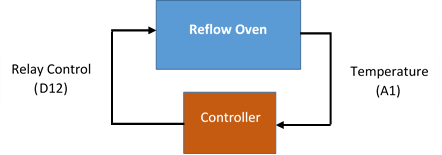
\includegraphics[width=0.7\textwidth]{fig1.png}
    \caption{Reflow Oven Controller}
\end{figure}

\par The best way to approach a more complex task like this is to make your program modular. A modular program intelligently subdivides a larger goal into small tasks. These small tasks can each be easily accomplished by writing a function. For example, you might create functions that implement the common tasks in your program (updating the LCD, calling user for inputs, etc). Modular programs offer many advantages, such as being much easier to debug (and easier to grade, incidentally!). 

\par
\indent
We will approach this control system as a multipart task which requires the construction of several functions. Each function may be tested individually and then integrated to achieve the overall goal of controlling a reflow oven.

\par \textbf{Objective 1:} Write a function that will control the state of the heater based on the current temperature. If the temperature is below the set point, turn the heater on. If the temperature is above the set point, then turn the heater off. The heater is controlled by pin D3 and the temperature is sensed at pin A5. Implement this logic and give your function a sensible name. If you have questions about converting the voltage read at pin A5 to a temperature, refer to the Thermocouple Tutorial document. Since room temperature calibration is available to you, the most important piece of information is that the transfer function of the thermocouple circuit has a response of approximately 5 mV / 1 C.

\par \textbf{Objective 2:} Amend the function from Objective 1 to include safety features in the event of a very high temperature, say 300 C. Your oven should never reach 300 C under any normal circumstances. What actions should you take if your oven reaches such a high temperature? Print messages to the user that will instruct them to handle this situation. Even if hardware based fail-safes are in place, robust software can add a layer of safety to the instrument. This is a critical aspect of medical device design.

\par 
\indent
The next step is to write functions that will allow the user to interact with the control system. Think back to the baby incubator lab in which you added front panel functions that permitted the user to adjust the set point of the baby incubator. We want to add this function to our temperature controller. We have five buttons to work with. Think about the most logical way to allocate these buttons to allow the user to select a temperature value.

\par
\textbf{Objective 3:} Write a function that will prompt the user to adjust the set point of the temperature controller. This function should allow the user to increment or decrement the temperature. This function should also test the set point as part of a ‘sanity check’ to see if the user set point is within a reasonable range (i.e. not unreasonable high and not below room temperature).

\par \textbf{Objective 4:} Write a function that will display the current temperature while the control algorithm is running. Keep in mind that a 2X16 LCD requires concise expressions. Also, print the set point temperature which the controller is trying to reach. 

\par 
\indent Now we will integrate the previous functions and test them with a suitable replacement system. A suitable test system can replace the temperature measurement with a potentiometer and an LED for the digital control output that would otherwise connect to the solid state relay terminal. 

\subsection*{\textbf{EEPROM}}
The EEPROM is non-volatile memory that can store information even when the Arduino is turned off, like the hard drive on your computer. This may be a good place to store long-term data and statistics that you can access every time you want to run the oven. Here are the three tutorials that help you get started, one for writing, and one for reading. Make sure you are comfortable with them since you will probably want to use it at some point in your project.
\begin{itemize}
\item \url{http://arduino.cc/en/Tutorial/EEPROMWrite} 
\item \url{http://arduino.cc/en/Tutorial/EEPROMRead}
\item \url{http://arduino.cc/en/Tutorial/EEPROMClear}

\end{itemize}
\end{document}
